\section{Experimental Methods} \label{sec:experiment}

In this section, you should provide a description of your experimental equipment, including enough detail for the reader to understand not only the physical layout but also the usage of the equipment.

\begin{figure}[ht]
    \centering
    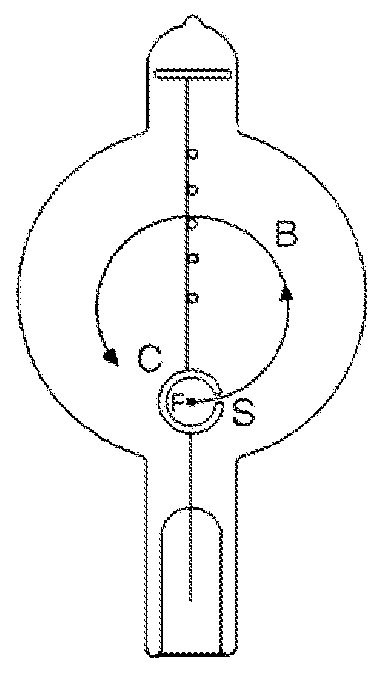
\includegraphics[width=0.4\linewidth]{figures/evacuated_tube.png}
    \caption{\footnotesize The evacuated tube used to measure the orbit radius of the electron beam in an external magnetic field. Electrons emitted by the filament (F) are collimated by a slit (S) and form a narrow beam (B). The crossbar (C) contains five markers at known orbit radii.}
    \label{fig:evacuated_tube}
\end{figure}

Present a figure showing the essential features of the apparatus early in this section, usually as a schematic drawing rather than a photograph. Refer to this figure within your text as Fig. 1; for example: A schematic representation of the apparatus used to measure the electron charge-to-mass ratio is shown in Fig. \ref{fig:evacuated_tube}. Then, locate this figure close to the text in which it is referenced. Notice that each figure contains a caption which provides a useful explanation of the figure's contents. Typically, figure and table captions use 10-point font.